\documentclass[10pt]{article}
\usepackage[letterpaper,margin=0.8in]{geometry}
\usepackage[T1]{fontenc}
\usepackage{lmodern,amsmath,booktabs,graphicx,caption,float,microtype}
\usepackage[colorlinks=true,urlcolor=blue,linkcolor=black]{hyperref}
\setlength{\parindent}{0pt}
\setlength{\parskip}{4pt}
\captionsetup{font=small,labelfont=bf}
% Generated by code/question2.py
\newcommand{\QTwoRawRows}{1,114,194}
\newcommand{\QTwoPanelRows}{1,105,619}
\newcommand{\QTwoPanelBanks}{17,620}
\newcommand{\QTwoOtherCharterRows}{8,575}
\newcommand{\QTwoInvalidAssetRows}{31}
\newcommand{\QTwoNonfiniteCashRows}{30}
\newcommand{\QTwoNegativeCashRows}{0}
\newcommand{\QTwoCashAboveAssetsRows}{1}
\newcommand{\QTwoInvalidRatioRows}{32}
\newcommand{\QTwoValidRatioRows}{1,105,587}
\newcommand{\QTwoUnavailableDiffRows}{17,789}
\newcommand{\QTwoUsableRows}{1,087,830}
\newcommand{\QTwoTooFewBanks}{7,060}
\newcommand{\QTwoRankDeficientBanks}{0}
\newcommand{\QTwoEstimatedBanks}{10,560}
\newcommand{\QTwoEstimationRows}{949,122}
\newcommand{\QTwoValidTests}{10,560}
\newcommand{\QTwoUnavailableTests}{0}
\newcommand{\QTwoSignificantBanks}{755}
\newcommand{\QTwoUnavailableFitStatistics}{0}
\newcommand{\QTwoMeanBeta}{-0.210}
\newcommand{\QTwoMedianBeta}{-0.158}
\newcommand{\QTwoMedianSE}{0.378}
\newcommand{\QTwoSignificantShare}{7.1}
\newcommand{\QTwoMedianRSquared}{0.046}
\newcommand{\QTwoMedianAdjustedRSquared}{-0.003}
\newcommand{\QTwoFirstMeanCash}{7.903}
\newcommand{\QTwoLastMeanCash}{9.404}

\begin{document}
\begin{center}\Large Question 2: Policy-rate changes and banks' cash shares\end{center}

\section*{1. Question and motivation}
I ask this question because the relationship between short-term interest rates and cash or reserve holdings is a straightforward mechanism often discussed in introductory monetary and macroeconomics courses. I am interested in how much explanatory power this relationship retains in real markets, where banks face complex conditions and unexpected shocks. Specifically, how much of the quarterly variation in commercial banks' cash-to-assets ratios is associated with current and recent federal funds rate changes during 1984--2017? I use Question 1's bank-specific regression structure and report model fit alongside sensitivity estimates.

\section*{2. Data, construction and estimation}
The only data inputs are \texttt{callreports\_1984\_2017.dta} and \texttt{FedFunds.csv}, both supplied for Question 1. The bank file labels \texttt{cash} as ``Cash and balances due from depository institutions.'' It includes more than reserves at the Federal Reserve; the outcome is therefore a broad cash-and-bank-balances share.\footnote{The corresponding reporting category includes currency, collection items and balances at other banks and the Federal Reserve: \href{https://www.chicagofed.org/banking/financial-institution-reports/fr2644-field-information}{Federal Reserve Bank of Chicago, FR 2644 field information, item 1}. The supplied file's label identifies the variable used here.} Both cash and total assets are reported in nominal USD thousands, so their units cancel in the ratio.

The script applies the following rules in order:
\begin{enumerate}
\item \textit{Keys and dates.} Read \texttt{idrssd}, \texttt{year}, \texttt{qdate}, \texttt{charter\_type}, \texttt{cash} and \texttt{total\_asset}; sort by bank and quarter. Require nonmissing, positive integer bank identifiers, integer quarter codes from 96 to 231 (1984Q1--2017Q4), \(year=1960+\lfloor qdate/4\rfloor\), and unique bank--quarter keys. A failed check stops execution; duplicates are not arbitrarily retained or averaged. These checks pass for \QTwoRawRows{} source rows.

\item \textit{Commercial-bank sample.} Retain rows with \texttt{charter\_type=200}; exclude \QTwoOtherCharterRows{} other or unclassified rows. This leaves \QTwoPanelRows{} rows for \QTwoPanelBanks{} banks. Cash availability is assessed independently of the income, expense and ROA samples from Question 1. Banks need not be listed companies.

\item \textit{Cash share.} Require finite \texttt{total\_asset}>0 and finite \(0\leq cash\leq total\_asset\). Set the ratio to missing if either condition fails, retaining the row for the audit. There are \QTwoInvalidAssetRows{} rows with invalid assets and \QTwoNonfiniteCashRows{} with nonfinite cash; these counts can overlap. There are \QTwoNegativeCashRows{} finite negative cash values and \QTwoCashAboveAssetsRows{} cash values above finite assets; the latter flag is a zero-assets observation already counted as invalid. In total, \QTwoInvalidRatioRows{} ratios are unavailable and \QTwoValidRatioRows{} are usable. Calculate
\[
 c_{it}=100\frac{cash_{it}}{total\_asset_{it}}.
\]
Zero cash and cash equal to assets remain valid. These are quarter-end balance-sheet stocks: use total assets, not quarterly average assets, and apply neither YTD subtraction nor annualization. Unlike Question 1's outcome rates, shares are not winsorized: values inside the accounting bounds are retained. This avoids another arbitrary cutoff, although unusual values within the bounds can still reflect errors.

\item \textit{Quarterly changes.} Within each bank, calculate \(\Delta c_{it}=c_{it}-c_{i,t-1}\) only when both ratios exist and their quarter codes differ by exactly one. Both records must survive the commercial-bank restriction. Q4-to-Q1 changes are allowed; the first record, missing inputs and gaps produce missing changes. Negative changes are valid declines. There is no interpolation, replacement of missing values, or balanced-panel requirement. This leaves \QTwoUnavailableDiffRows{} observed rows without a usable change. With no pre-1984 bank data, estimation starts no earlier than 1984Q2.

\item \textit{Policy rate and merge.} Reuse Question 1's \texttt{f\_construction()}: take the monthly effective federal funds rate in March, June, September and December, in percent. Match one-to-one to a complete 1983Q1--2017Q4 calendar; duplicate quarters, unmatched dates, missing rates or rates outside \([0,100)\) stop execution. Construct \(\Delta f_t=f_t-f_{t-1}\) and its three quarterly lags before restricting to 1984--2017. Left-merge onto bank observations using \texttt{qdate}, requiring many-to-one matching and a policy match for every bank row. The policy calendar is complete; gaps in bank histories never alter policy-lag distances.

\item \textit{Regression eligibility.} Keep rows with finite \(\Delta c\) and all four policy regressors: \QTwoUsableRows{} bank--quarters before the minimum-history rule. Each bank needs at least 40 such observations and design-matrix rank five. Quarters need not be consecutive. The 40-quarter cutoff is inherited from Question 1 and remains arbitrary; no new cutoff search is performed. The audit identifies \QTwoTooFewBanks{} banks with insufficient observations and \QTwoRankDeficientBanks{} remaining banks with deficient rank. Estimate \QTwoEstimatedBanks{} banks using \QTwoEstimationRows{} observations in total.
\end{enumerate}

For each eligible bank, fit ordinary least squares:
\[
\Delta c_{it}=a_i+\sum_{j=0}^{3}b_{ij}\Delta f_{t-j}+u_{it},
\qquad \widehat\beta_i=\sum_{j=0}^{3}\widehat b_{ij}.
\]
Each usable quarter has equal weight within a bank; each estimated bank has equal weight in the summaries. The intercept permits a bank-specific average change. Differencing removes constant differences in cash-share levels. Full calendar-quarter fixed effects would give each date (1984Q1, 1984Q2, and so on) its own intercept. Since each bank has one observation per date, these effects would fit every observation separately and absorb all four policy regressors, leaving their coefficients unidentified. They are therefore omitted. No additional controls, subgroup regressions or cross-sectional second-stage regressions are added.

Beta excludes the intercept and measures the associated cumulative cash-share change over the current and following three quarters for a one-percentage-point policy-rate increase, holding other policy changes fixed. To describe fit, calculate
\[
R_i^2=1-\frac{\sum_t\widehat u_{it}^{\,2}}
 {\sum_t(\Delta c_{it}-\overline{\Delta c_i})^2},
\qquad
\overline R_i^2=1-(1-R_i^2)\frac{n_i-1}{n_i-5}.
\]
The first measures in-sample variation accounted for by the four policy regressors beyond an intercept. The second adjusts for fitting five parameters; negative adjusted values are retained. Neither statistic measures causal explanatory power or forecasting performance.

Inference follows Question 1: Bartlett HAC covariance through four actual calendar-quarter lags, correction \(n_i/(n_i-5)\), and a two-sided asymptotic normal Wald test of \(H_0:\sum_j b_{ij}=0\). The beta variance sums the entire four-by-four slope covariance block, including covariances. A constant outcome or nonpositive/nonfinite beta variance receives unavailable inference; a constant outcome also has unavailable fit statistics. Point estimates remain in the distribution. Median SE and the significant share use only tests with status \texttt{ok}, finite positive SE and \(p\in[0,1]\); significance means \(p<0.05\). Tests are unadjusted for multiple comparisons. This tests the slope sum, not the joint hypothesis that every lag coefficient is zero, and supplies no test of the mean beta across banks.

\section*{3. Evidence}
\begin{table}[H]
\centering
\caption{Bank-level cash-share responses and model fit}
\begin{tabular}{lr}
\toprule
Metric & Value \\
\midrule
Eligible banks & 10,560 \\
Mean cumulative beta & -0.210 \\
Median cumulative beta & -0.158 \\
Median HAC standard error & 0.378 \\
Banks with cumulative $p<0.05$ (\%) & 7.1 \\
Median $R^2$ & 0.046 \\
Median adjusted $R^2$ & -0.003 \\
\bottomrule
\end{tabular}

\begin{minipage}{0.9\textwidth}\footnotesize
Equal bank weights. Beta units are cash-share percentage points per policy-rate percentage point. Median HAC SE is the median uncertainty of individual bank betas, not the SE of the mean or median beta. Significant shares exclude \QTwoUnavailableTests{} unavailable tests. Fit statistics describe quarterly changes, with an intercept in every regression.
\end{minipage}
\end{table}

The mean cumulative beta is \QTwoMeanBeta{} and the median is \QTwoMedianBeta{}. A one-percentage-point policy-rate increase is associated with a cumulative cash-share change of \QTwoMeanBeta{} percentage points for the average eligible bank, under the fitted model. Across banks, the median \(R^2\) is \QTwoMedianRSquared{}: the model accounts for about 4.6\% of within-bank variation in quarterly cash-share changes at the median. Median adjusted \(R^2\) is \QTwoMedianAdjustedRSquared{}, indicating weak fit after accounting for the four policy slopes. The share of available bank tests rejecting a zero cumulative association is \QTwoSignificantShare{}\%. Economic magnitude, model fit and statistical significance address different questions; lag coefficients can offset in the cumulative sum even when they help fit the data.

\begin{figure}[H]
\centering
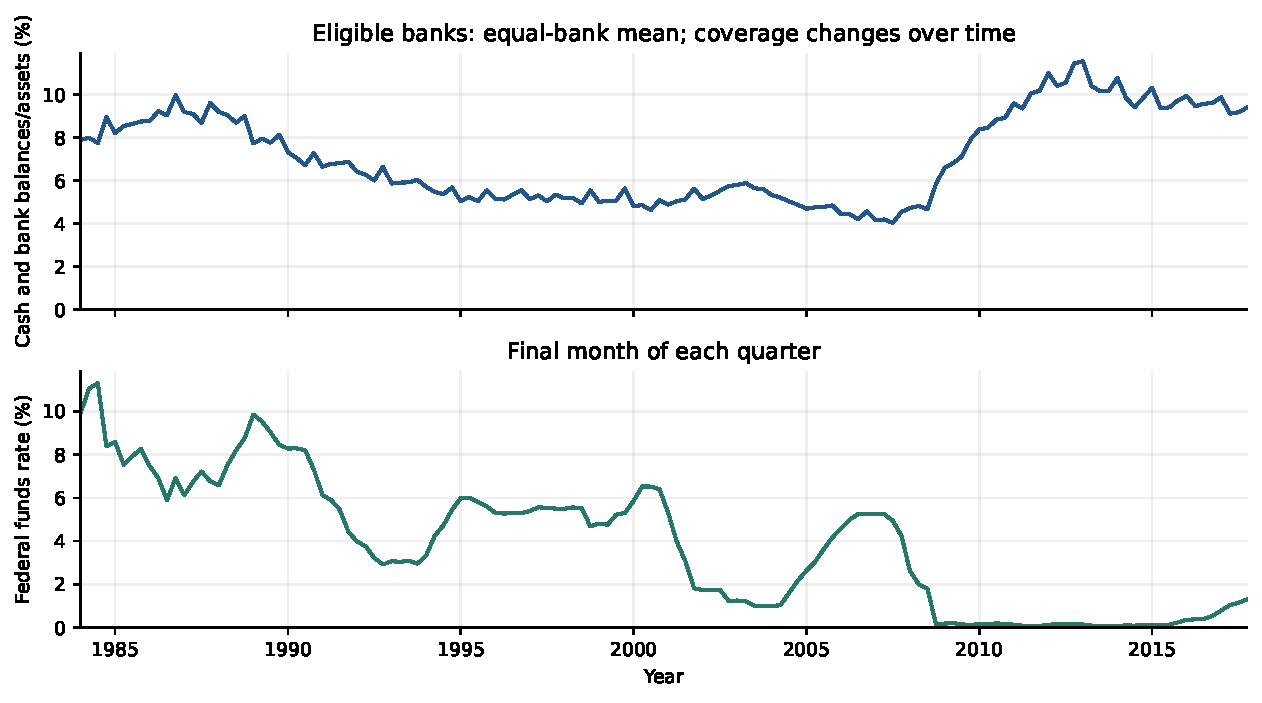
\includegraphics[width=0.82\textwidth]{figures/question2_cash.pdf}
\caption{Cash shares and the federal funds rate. The upper panel averages valid cash shares equally across regression-eligible banks observed in each quarter; the lower panel uses the quarter's final monthly policy rate. The available bank composition changes over time. These level series provide context; the regressions use bank-level changes.}
\end{figure}

The plotted mean cash share is \QTwoFirstMeanCash{}\% in 1984Q1 and \QTwoLastMeanCash{}\% in 2017Q4. This describes available eligible banks, not an asset-weighted industry ratio or the evolution of a fixed bank cohort.

\section*{4. Interpretation and limitations}
The negative average response is consistent with banks reducing their cash share as policy rates rise, but the low fit statistics indicate limited explanatory power. This does not by itself reject the textbook mechanism: the outcome is broader than Fed reserves, and the model describes association rather than an identified policy effect.

I do not control for major macroeconomic events, including recessions and financial crises, which can affect both policy rates and banks' cash holdings. The introduction of interest on reserve balances in October 2008 may also change the relationship over time.\footnote{\href{https://www.federalreserve.gov/newsevents/pressreleases/monetary20081006a.htm}{Federal Reserve announcement, October 6, 2008}.} Nor do I explicitly model banks' different business focuses, such as lending mix, deposit funding and payment services, or changes in those activities. Separate bank intercepts and slopes allow different average changes and estimated responses, but do not explain the sources of those differences or control for changing business conditions.

I also do not construct each bank's minimum required reserves or account for regulatory changes during the sample. Requirements depended on the types and amounts of reservable liabilities, with exemptions, thresholds and ratios that changed over time; banks with different funding structures could therefore face different requirements.\footnote{Federal Reserve \href{https://www.federalreserve.gov/monetarypolicy/rmm/Chapter_3_Calculation_of_Reserve_Balance_Requirements.htm}{Reserve Maintenance Manual} and \href{https://www.federalreserve.gov/monetarypolicy/reservereq.htm}{historical reserve requirements}.} The broad cash/assets ratio is not a measure of compliance with those requirements.

Ratio changes can reflect either cash or total assets; entry, exit, mergers and differing bank histories affect comparability. HAC standard errors address heteroskedasticity and serial correlation, not omitted-variable bias, and may be unreliable with short histories. Nominal significant shares also face multiple-testing concerns and correlated bank outcomes.

\paragraph{Time spent.} 3 hours.
\end{document}
